\documentclass[border=2pt]{standalone}
\usepackage{tikz}
\usetikzlibrary{arrows.meta,chains,%
                    decorations.pathreplacing}
\usetikzlibrary{matrix,positioning,arrows.meta,arrows}

\tikzset{
mymat/.style={
  matrix of nodes,
  nodes in empty cells,
  text height=2.5ex,
  text depth=0.75ex,
  text width=3.25ex,
  align=center,
  column sep=-\pgflinewidth
  }
}
\tikzset{
  rows/.style 2 args={
    sub@rows/.style={row ##1 column #2/.style={nodes={rectangle,draw=black}}},
    sub@rows/.list={#1}
  },
  box/.style 2 args={
    sub@box/.style={rows={#1}{##1}},
    sub@box/.list={#2}
  }
}
\begin{document}

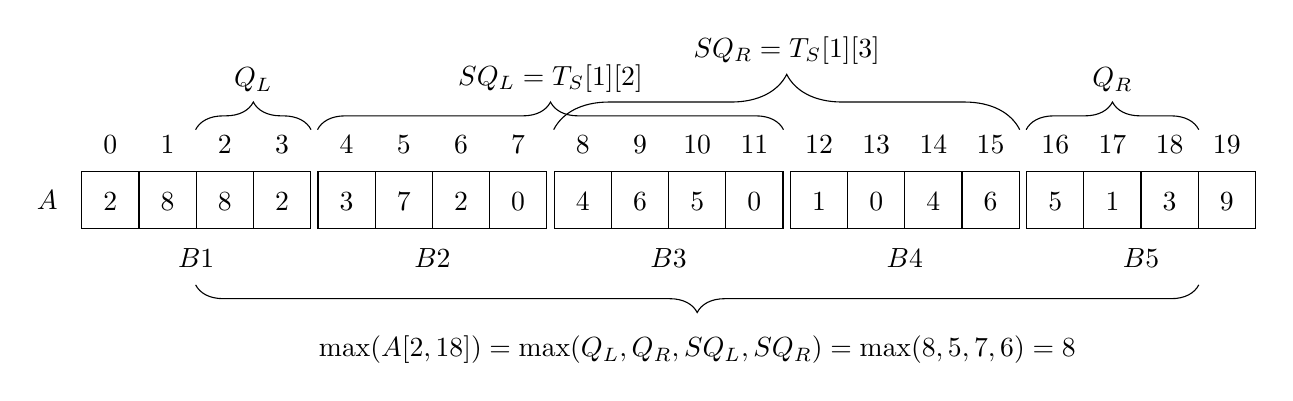
\begin{tikzpicture}[>=latex]
\matrix[mymat,anchor=west,
    box={2}{1, 2, 3, 4}]
at (0,0) 
(mat1)
{ 
  0 & 1 & 2 & 3 \\
  2 & 8 & 8 & 2 \\ };
\matrix[mymat,anchor=west,
    box={2}{1, 2, 3, 4}]
at (3,0) 
(mat2)
{ 4 & 5 & 6 & 7 \\
  3 & 7 & 2 & 0 \\ };
\matrix[mymat,anchor=west,
    box={2}{1, 2, 3, 4}]
at (6,0) 
(mat3)
{ 8 & 9 & 10 & 11 \\
  4 & 6 & 5 & 0 \\ };
\matrix[mymat,anchor=west,
    box={2}{1, 2, 3, 4}]
at (9,0) 
(mat4)
{ 
  12 & 13 & 14 & 15 \\
  1 & 0 & 4 & 6 \\ };
\matrix[mymat,anchor=west,
    box={2}{1, 2, 3, 4}]
at (12,0) 
(mat5)
{ 16 & 17 & 18 & 19 \\
  5 & 1 & 3 & 9 \\ };

\node[left=5pt of mat1-2-1.west]
{
   $A$ \\
};
\node[below=0pt of mat1]{$B1$};
\node[below=0pt of mat2]{$B2$};
\node[below=0pt of mat3]{$B3$};
\node[below=0pt of mat4]{$B4$};
\node[below=0pt of mat5]{$B5$};

\draw[decorate,decoration={brace, amplitude=10pt, raise=20pt, mirror}]
  (mat1-2-3.south west) to node[black,midway,below= 35pt] {$\max(A[2, 18]) = \max(Q_L, Q_R, SQ_L, SQ_R) = \max(8, 5, 7, 6) = 8$} (mat5-2-3.south east);

\draw[decorate,decoration={brace, amplitude=10pt, raise=15pt}]
  (mat1-2-3.north west) to node[black,midway,above=25pt] {$Q_L$} (mat1-2-4.north east);

\draw[decorate,decoration={brace, amplitude=10pt, raise=15pt}]
  (mat5-2-1.north west) to node[black,midway,above=25pt] {$Q_R$} (mat5-2-3.north east);

\draw[decorate,decoration={brace, amplitude=10pt, raise=15pt}]
  (mat2-2-1.north west) to node[black,midway,above=25pt] {$SQ_L = T_S[1][2]$} (mat3-2-4.north east);

\draw[decorate,decoration={brace, amplitude=20pt, raise=15pt}]
  (mat3-2-1.north west) to node[black,midway,above=35pt] {$SQ_R = T_S[1][3]$} (mat4-2-4.north east);
\end{tikzpicture}

\end{document}